\documentclass[border=1pt]{standalone}
\usepackage{tikz}
\usepackage{luatexja}
\usetikzlibrary{shapes.geometric, backgrounds}

\begin{document}
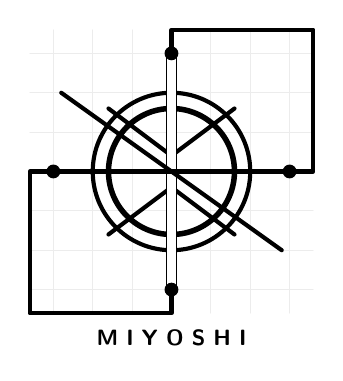
\begin{tikzpicture}[line width=1.5pt, line cap=round, line join=round]
    % 背景グリッド
    \begin{scope}[gray!15, line width=0.3pt]
        \foreach \i in {-1.5, -1, ..., 1.5} {
            \draw (\i, -1.8) -- (\i, 1.8);
            \draw (-1.8, \i) -- (1.8, \i);
        }
    \end{scope}

    % 外枠
    \draw (0,0) rectangle (1.8, 1.8);
    \draw (0,0) rectangle (-1.8, -1.8);

    % M, I, Y, O, S, H, I の統合
    \draw[line width=2pt] (0,0) circle (0.8); % O
    \draw (0,0) circle (1.0); % 装飾外円
    
    % M & Y (上下のV字)
    \draw (-0.8, 0.8) -- (0, 0.2) -- (0.8, 0.8);   % MのV
    \draw (-0.8, -0.8) -- (0, -0.2) -- (0.8, -0.8); % YのV
    
    % H & I (垂直・水平軸)
    \draw[double, double distance=3pt, line width=0.5pt] (0, -1.5) -- (0, 1.5); % I
    \draw (-1.2, 0) -- (1.2, 0); % H横棒
    
    % S (斜めの鋭い貫通線)
    \draw (-1.4, 1.0) -- (1.4, -1.0);

    % 端点の装飾
    \foreach \angle in {0, 90, 180, 270} \fill (\angle:1.5) circle (2.5pt);

    % テキスト
    \node[anchor=north, font=\sffamily\bfseries, scale=0.8] at (0, -1.9) {M I Y O S H I};
\end{tikzpicture}
\end{document}
